\documentclass[11pt, fleqn]{article}
\usepackage{graphics, graphicx, color, amsmath, natbib}
\textwidth17cm
\textheight20cm
\topmargin0in \oddsidemargin  0 in \evensidemargin  0 in
\setlength{\parindent}{0.0in}
\newfont{\Bb}{msbm11}
\newcommand{\real}{\mbox{\Bb R}}

\bibpunct{(}{)}{,}{a}{}{;}
\begin{document}
\begin{center}
{\LARGE Bayesian Melding in Urban Simulations}\\[3mm]
Hana \v{S}ev\v{c}\'{\i}kov\'{a}, Adrian Raftery and Paul Waddell\\
University of Washington\\[5mm]
Draft\\
\today
\end{center}

{\bf Abstract:}

\vspace{1cm}

\section{Introduction}
\label{sec:Intro}
%
\begin{itemize}
\item Simulation of processes in environmental disciplines often provide
  point results. 
\item The need of expressing uncertainty of such results widely recognized
  (\citet{refsgaard04}, \citet{vanasselt02}).
\item Great deal of work in terms of uncertainty in hydrology and high risk
  areas (\citet{beven92}, \citet{beven00}, \citet{christensen03}, \citet{neuman03},
  \citet{korving03}).
\item Work on the whaling project (\citet{raftery95}, \citet{poole00}). 
\item Application to UrbanSim (\citet{waddell02}, \citet{waddell03}).
\end{itemize}

\section{UrbanSim}
\subsection{Description}
%
\label{sec:US-description}
UrbanSim is an urban simulation model operational in several urban areas in
the United States (\citet{waddell02}, \citet{waddell03}). The system is
implemented as a set of interacting models that represent the major actors and
choices in the urban system, including household moving in a residential
location, business choices of employment location and developer choices of
locations and types of real estate development. It is taking an extremely
disaggregated approach by modeling individual households, jobs, and real
estate development and location choices using grid cells of $150\times 150$
meters in size. The model system microsimulates the annual evolution in
locations of individual households and jobs, end the evolution of the real
estate within each individual grid cell as the result of actions by real
estate developers. 

In this section, we give a brief description of the main components of the
system. Our emphasis is less on the details of the algorithms of the
individual models, but rather on the information on which models base their
procedures.  For details about the algorithms see \citet{waddell03}.

The core of UrbanSim consists of nine models that run in a certain order once
per a simulated year. In Figure~\ref{fig:urbansim}, the models are sorted
from top to bottom according to their run order. Models that are placed on
the same horizontal level are independent of each other. 


\begin{figure}[t]
\begin{center}
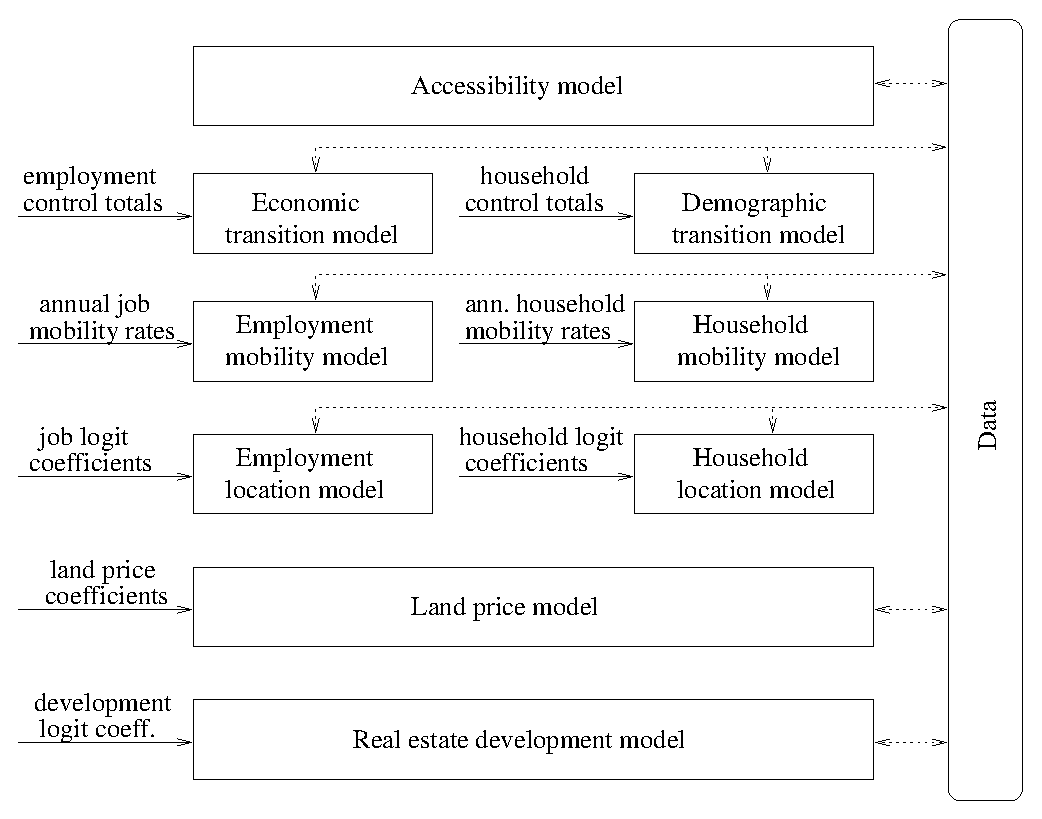
\includegraphics[scale=0.8]{pic/UrbanSim.eps}
\caption{\label{fig:urbansim}\small UrbanSim models in order of their runs
  (from top to bottom). The solid arrows show external input parameters, the
  dash arrows mark the data flow.}
\end{center}
\end{figure}



A simulation is usually performed for a certain time period given in number of
years. It is expected that at the beginning of the simulation, data reflect
the true state in the starting year. We will call such data 'base year' data.
Each model uses a certain partition of the data as an input and modifies a
certain partition of the data according to the results of the run of this
particular model. These relations are represented in Figure~\ref{fig:urbansim}
by dashed arrows. Moreover, most of the models expect additional input
parameters (see bellow) that are marked by solid arrows.

The simulation starts by running the {\bf Accessibility model}. This model
creates accessibility indices that summarize the accessibility from a given
geographical unit to various activities. The indices are then used in
Employment and Household location models where accessibilities are expected to
influence household or business choice of location. The Accessibility model is
loosely coupled with a Travel model (not included in the figure) that is for
simplicity considered here as an external model.

The {\bf Economic transition model} simulates job creation and loss. It uses
aggregate employment forecasts (control totals) that are obtained from
external sources (state economic forecasts, commercial or in-house sources).
Analogously, the {\bf Demographic transition model} simulates births and
deaths in the population of households. Here again, control totals from
aggregated forecasts obtained from external sources are used as an additional
input.

The {\bf Employment mobility model} determines which jobs will move from their
current locations during the simulated year. It uses annual mobility rates
directly observed over a recent period. They are computed from longitudinally
linked business establishment files. Similarly, the {\bf Household
  mobility model} simulates households deciding whether to move. The algorithm 
uses annual mobility rates estimated from the Census Current Population
Survey. 

The {\bf Employment location choice model} is responsible for determining a
location for each job that was either newly created or determined for
moving. The  {\bf Household location choice model} chooses a location for each
household that was either created or belongs to the mover set. Both models are
based on a multinomial logit model calibrated to observed data. Thus,
logit coefficients are required by the models as additional input
parameters. These coefficients are usually estimated by external estimation
procedures.  

The {\bf Land price model} simulates land prices of each grid cell as the
characteristics of locations change over time. It is based on a hedonic
regression~\citep{waddell93} using coefficients estimated externally from
historical data. 

The one year simulation is concluded by the {\bf Real estate development
  model} that simulates developer choices about what kind of construction to
undertake and where. It uses the multinomial logit model and here again, its
coefficients are estimated externally using observed data.

\subsection{Sources of uncertainty}
%
In order to make a probabilistic analysis of any system, the first step is to
identify all possible sources of uncertainty of this system (see e.g.
\citet{morgan90}, \citet{dubus03}, \citet{regan03}). The goal of the analysis
is then to quantify as much of the identified uncertainty as possible.

This section reviews sources of uncertainty that are entering UrbanSim.

\subsubsection{Measurement errors}
%
As mentioned above, data that enter UrbanSim at the beginning of any
simulation run (base year data) should reflect the true state of the world.
The data are collected from different sources, such as census or commercial
sources. Obviously, such data are subject to errors, moreover, they often
contain missing values. For example, concerning parcel data, tax exempt
properties like government-owned properties tend to have very incomplete data
in the assessor files, since there is no compelling reason for assessors to
collect these items.  These data are massive in volume, and rely on individual
property assessors to input data, and the resulting databases are often
riddled with missing data and data errors. As a result, it is in user
responsibility to deal with these limitations, for example by applying
imputation procedures. 

\subsubsection{Systematic errors}
%
Systematic errors is a type of uncertainty that can bias the simulation
results. It arises for example due to wrongly calibrated measurement tools or
due to not completely random sampling procedures. An example of the latter
case would be a situation where households belonging to a certain category,
such as a certain race, are excluded from the sampling process when creating
the household database from census sources. Both, the measurement errors and
the systematic errors affect the quality of the base year data.

\subsubsection{Uncertainty in model structure}
%
In this category, three types of uncertainty can be distinguished. First, the
selection of variables that are entering the statistical models embedded in
UrbanSim, such as the multinomial logit model or the hedonic regression.
Second, the choice of the statistical model itself. For example, processes
modelled by the multinomial logit could be modelled by other model of the
discrete choice model family, such as the multinomial probit or mixed logit
model~\citep{train03}. Third type of uncertainty in this category arises
through the selection of the processes that are modelled by UrbanSim. It is
obvious that the collection of UrbanSim models does not represent a complete
set of processes that in real life influence the evolution in households and
jobs locations.  Therefore, since the UrbanSim system represent only an
abstraction of all real life processes that affect the modelled quantities, it
is subject to uncertainty.

\subsubsection{Uncertainty in model input parameters}
%
As described in Section~\ref{sec:US-description}, there are several sets of
input parameters that enter UrbanSim and all of them are estimated by external
models or procedures. Since they are estimates of some true values, they can
be used to make statistical inference and thus, can be included in the
uncertainty analysis of the simulation results.  

\subsubsection{Stochasticity}
%
An important source of uncertainty arises by using random numbers within
models. The fact that simulations with different seeds of the random number
generator will produce different results, has to be taken into account in the
uncertainty analysis. In UrbanSim, several models that use multinomial logit
model use a sampling procedure for sampling choice alternatives. Additionaly,
both mobility models use sampling for determining movers according to given
rates. 

Table~\ref{tab:models} summarizes for each model the information about the
main component of the procedure, the estimation of the input parameters, and
the fact if random numbers (RNs) are used by the model.

\begin{table}
\begin{center}
\begin{tabular}{|c||c|c|c|}\hline
model & procedure & estimation of input param. & RNs
\\\hline\hline
Accessibility & deterministic & -- & no \\\hline
Economic/Demographic & algorithmus based on &  &  \\
transition & joint prob. distr. & external sources & yes \\
& of jobs/households & & \\\hline
Employment/Household & random sampling & observed rates& yes\\
 mobility&&&\\\hline
Employment/Household & multinomial logit & multinomial logit & yes\\
location choice &&&\\\hline
Land price & hedonic regression & hedonic regression & no \\\hline
Development & multinomial logit & multinomial logit & yes\\\hline
\end{tabular}
\caption{\label{tab:models}\small Procedure type, type of estimation of input
  parameters and random numbers (RNs) usage for each model.}
\end{center}
\end{table}
\section{Method}
\label{sec:Method}
%
\subsection{Basic Notation}
%
Let the $D$-dimensional space of all possible model input parameters be
denoted by $\Theta^D \subset \real^D$.  A~model $M$ expects $\Theta^D_i
\subset \Theta^D$ as its input and generates output $\Phi^K_i \subset \Phi^K$.
Thus, $\Phi^K\subset\real^K$ denotes the $K$-dimensional space of all possible
model outputs. For simplicity, we omit the superscript and write $\Theta$,
$\Theta_i$, $\Phi$ and $\Phi_i$, respectively. Now, we can write $\Phi_i =
M(\Theta_i)$, or more generally $\Phi = M(\Theta)$.

$M$ is considered as a simulator that starts at time $t_0$ in a certain state
and simulates given processes until time $t_2$. Thus, $\Phi$ is related to a
certain time point, here $\Phi = \Phi(t_2)$.  The state at time $t_0$ is
usually based on observed data at $t_0$, denoted here by $y(t_0)$ ($y \subset
\real^K$). If observed data are available for some $t_1$ ($t_0 < t_1 < t_2$),
we can use $y(t_1)$ to assess a more precise shape of the output space $\Phi$.
The described scenario is shown in Figure~\ref{fig:BM}.

\begin{figure}
\begin{center}
\input{pic/BM.pstex_t}
\caption{\label{fig:BM}\small }
\end{center}
\end{figure}

\subsection{Formulation}
%
We define our quantities of interest $\psi$ as a function of model
outputs: 
\[
\psi = \Psi(\Phi) = \Psi(M(\Theta))\,.
\]

Let $q(\Theta)$ denote the prior distribution of $\Theta$.  The likelihood of
simulated outputs is 
\begin{equation}
\label{eq:likelihood}
L(\Phi) = prob(y | \Phi)\,.
\end{equation}
Then the posterior
distribution of inputs can be written as
\[
p(\Theta) \propto q(\Theta)L(\Phi)
\]
which can be translated into a posterior distribution of model outputs and
quantities of interest.

\subsection{Simulating posterior distribution}
\label{sec:simupost}

In \citet{raftery95} and \citet{poole00} a method called Bayesian
melding has been proposed which puts analysis of simulation models on a solid
statistical footing. It provided a purely deterministic model with a Bayesian
framework in order to assess uncertainty about the natural rate of increase of
bowhead whales. 

The method is based on Monte Carlo simulation and can be discribed in a
simplified way as follows:
\begin{enumerate}
\item Draw a sample $\{\Theta_1,\dots,\Theta_I\}$ of values of the inputs from
  the prior distribution $q(\Theta)$.
\item  Obtain $\{\Phi,\dots,\Phi_I\}$ where
  $\Phi_i = M(\Theta_i)$. 
\item Compute weights $w_i = L(\Phi_i)$. As a result, we get an approximate
  posterior distribution of inputs with values $\{\Theta_1,\dots,\Theta_I\}$
  and probabilities proportional to $\{w_1,\dots,w_I\}$. 
\item The approximate posterior distribution of the quantities of interest has
  values $\{\psi_1,\dots,\psi_I\}$ where $\psi_i=\Psi(\Phi_i)$ and
  probabilities proportional to $\{w_1,\dots,w_I\}$.
\end{enumerate}

The applications that we are dealing in this paper with are not
deterministic. We consider here models that contain a stochastic component in
terms of using random numbers. Runs with different seeds return different
results. To include this source of uncertainty into the framework, we modify
the above procedure as follows:

\begin{enumerate}
\item As above.
\item  For each $\Theta_i$, run the model $J$ times with different seeds to
  obtain $\Phi_{ij}, j=1,\ldots,J$.
\item Compute weights $w_i = L(\bar{\Phi}_{i})$ where
  $\bar{\Phi}_{i}=\frac{1}{J}\sum_{j=1}^J \Phi_{ij}$. Here again, we get an
  approximate posterior distribution of inputs with values
  $\{\Theta_1,\dots,\Theta_I\}$ and probabilities proportional to
  $\{w_1,\dots,w_I\}$.
\item $\psi$ now has a distribution given $\Theta_i$.
\end{enumerate}


\subsection{Likelihood}
%
In order to compute the weights in Step~3 of Section~\ref{sec:simupost}, we
need to define a likelihood function (Eq.~\ref{eq:likelihood}). Specifically,
\begin{equation}
w_i \propto p(y|\Theta_i) = \prod_{k=1}^K p(y_k | \Theta_i)\,.
\end{equation}

Assessing $p(y|\Theta_i)$ is based on the following model:
\begin{eqnarray}
\Phi_{ijk} & = & \mu_{ik} + \delta_{ijk}, \text{ where } \delta_{ijk}
\stackrel{iid}{\sim} N(0,\sigma_{\delta}^2) \label{eq:phi}\\
(y_{k}|\Theta=\Theta_i) & = & \mu_{ik} + a + \epsilon_{ik}, \text{ where } \epsilon_{ik}\stackrel{iid}{\sim} N(0,\sigma_{i}^2)\label{eq:y}
\end{eqnarray}
Here, $\mu_{ik}$ denotes the expected output for $\Theta_i$ and $k$-th
dimension of the output. Futhermore, $\delta_{ijk}$ and $\epsilon_{ik}$ denote
model errors and $a$ denotes the overall bias in the model.

Estimation of $\mu_{ik}$, $\sigma_{\delta}^2$, $\sigma_{i}^2$, and $a$
can be done by approximate maximum likelihood (see Appendix~\ref{app:est}). We
denote these estimates by $\hat{\mu}_{ik}$, $\hat{\sigma}_{\delta}$,
$\hat{\sigma}_{\epsilon}^2$ and $\hat{a}$, respectively.

This yields a predictive distribution of our quantity of interest:
\begin{equation}
\label{eq:yk}
y_k | \Theta_i \sim N(\hat{a} + \hat{\mu}_{ik}, v_i)\quad \text{with} \; v_i=\hat{\sigma}_i^2 + \frac{\hat{\sigma}_{\delta}^2}{J}\,.
\end{equation}
(see Appendix~\ref{app:postdistr} for details).

We then have
\begin{eqnarray}
w_i & \propto & p(y|\Theta_i) =  \prod_{k=1}^K \frac{1}{\sqrt{2\pi v_i}}
\exp\left[-\frac{1/2(y_k-\hat{a} - \hat{\mu}_{ik})^2}{v_i}\right] \quad \text{and}\label{eq:wi}\\
\log w_i & \propto  &-\frac{K}{2} \log(2\pi v_i) - \frac{1}{2v_i}\sum_{k=1}^K
(y_k-\hat{a} -\hat{\mu}_{ik})^2 \,.\label{eq:logwi}
\end{eqnarray}

\subsection{Posterior distribution of quantities of interest}
%
Given that $\hat{\sigma}_{\delta}$, $\hat{\sigma}_{\epsilon}^2$ and $\hat{a}$
were estimated at time point $t_1$, the marginal distributions of model
outputs for the time point $t_2$ are given by a mixture of normal
distributions
\begin{equation}
\label{eq:p-phi-marg}
p(\Phi_k) = \sum_{i=1}^I w_i N(\hat{a}b_a + \hat{\mu}_{ik}(t_2), (\hat{\sigma}_i^2 + \frac{\hat{\sigma}_{\delta}^2}{J})b_v)\,,\quad k=1,\dots,K
\end{equation}
where $b_a$ and $b_v$ denote propagation factors (over the time period $t_2 -
t_1$) of the bias and the variance, respectively.

The resulting posterior distribution of the quantity of interest $\psi$ is given by
\begin{equation}
\label{eq:p-psi}
p(\psi) = \sum_{i=1}^I w_i \left[\prod_{k=1}^K \Psi(N(\hat{a}b_a + \hat{\mu}_{ik}(t_2),(\hat{\sigma}_i^2 +
  \frac{\hat{\sigma}_{\delta}^2}{J})b_v))\right]\,.
\end{equation}



\section{Application}
\label{sec:App}
%
\subsection{Model}
%
In this section, we apply the described method to our test data. It consists
of data from the area of Eugene-Springfield, OR, in 1980. Our goal is to make
a prediction using UrbanSim for the year 2000. Specifically, our quantity of
interest $\psi$ is the spacial distribution of households in the considered
area (on the traffic analysis zone (TAZ) level or its aggregation).

As model outputs $\Phi$, we are interested in number of households per TAZ.
Thus, the number of traffic zones determines the dimension $K$ of our output
space, here $K=295$ (with possible reduction, see Section~\ref{sec:weights}).

For computing the weights (Eqs.~\ref{eq:wi} and \ref{eq:logwi}), we use
observed number of households in each zone in 1994, denoted here as
$y_1,\dots,y_K$.

%
\subsubsection{Prior on inputs}
%
Input parameters that were derived by the multinomial logit procedure or by
the hedonic regression (see Table~\ref{tab:models}) have known standard errors
(SE) and covariance matrices (C).  For these parameter sets we used the
multivariate normal distribution MVN$(\hat{\Theta},\text{C}((\hat{\Theta}))$
where $\hat{\Theta}$ is the parameter estimator of the true value $\Theta$.
Note that the values of the covariance matrices were negligible (except of the
diagonal) so that we used only diagonal matrices of
diag$(\text{SE}(\hat{\Theta})^2)$. 

For each mobility rate $r$ in the employment and household mobility models we
used the zero truncated normal distribution N$(\hat{r},
(\frac{\hat{r}(1-\hat{r})}{n})^2)$ where $\hat{r}$ is an estimation of the
true rate $r$ and $n$ is the number of observations from which $\hat{r}$ was
obtained.

In terms of the control totals for the economic and demographic transition
model, respectively, we obtained a predictions for the end year of the
simulation and interpolate these values to the years prior to the end year.
Additionally, we obtained several pairs of prediction and true observation
values from the historical data, in order to estimate the standard error on
these totals. Then we assigned each total $c$ with the normal distribution
N$(c,\text{SE}(c))$. {\em Should we say that our $c$ is the true value from
  2000?}.

\subsubsection{Simulation}
%
We run UrbanSim for $100$ different inputs, each of them twice with different
random seed.  That is $200$ runs in total, with $I=100$ and $J=2$. Note that
we confirmed our results on a simulation with $I=1000$ and $J=3$. Since an
UrbanSim simulation of this size is in practice not feasible due to the long
run time, in this paper we refer to results of the smaller simulation but
point to differences if any.

The simulation was started in 1980 and run until 2000. Results
$\Phi_{ijk}(1994)$ and $\Phi_{ijk}(2000)$ were saved for all $i=1,\dots,I$,
$j=1,\dots,J$, $k=1,\dots,K$.


\subsection{Results}
%
\subsubsection{Transformation}
%
In Equation~\ref{eq:phi} and~\ref{eq:y}, we are assuming that our model errors
have constant variances $\sigma_{\delta}^2$ over all $i$ and $k$, and
$\sigma_{\i}^2$ over all $k$.

In Figure~\ref{fig:mean-sd} we examine the relationship between the estimate
of $\Phi_{ijk}(1994)$, denoted by $\hat{\mu}_{ik}$, and its standard
deviation, sd($\Phi_{ijk}$). Obviously, sd($\Phi_{ijk}$) increases with
increasing $\hat{\mu}_{ik}$. The relationship is approximately linear on the
log-log scale, shown in the right panel of Figure~\ref{fig:mean-sd}.


\begin{figure}[t]
\begin{center}
\begin{minipage}{8cm}
\includegraphics[scale=0.3, angle=-90]{pic/hu_mean_sd_all.ps}
\end{minipage}
\hfill
\begin{minipage}{8cm}
\includegraphics[scale=0.3, angle=-90]{pic/hu_lmean_lsd_all.ps}
\end{minipage}
\caption{\label{fig:mean-sd}\small Scatter plot of $\hat{\mu}_{ik}$
  vs. standard deviation of $\Phi_{ijk}$ for $t=1994$ and the corresponding
  lowess curve (raw data in the left panel, data on the log-log scale in the
  right panel). The plots contain 500 randomly selected points from $I\cdot K
  = 29500$ points in total (excluding points where either $\hat{\mu}_{ik}$ or
  sd($\Phi_{ijk}$) is equal zero). The lowess curve is based on all points.}
\end{center}
\end{figure}

A detailed analysis of the slope suggested to transform the data on the square
root scale. Figure~\ref{fig:mean-sd-tran} shows the scatter plots from
Figure~\ref{fig:mean-sd} after the square root transformation. The
relationship became weak, in particular the squared correlation coefficient is
now $R^2 = 0.03$. Note that we excluded data from the analysis where either
$\hat{\mu}_{ik}$ or sd($\Phi_{ijk}$) is equal zero.

\begin{figure}[t]
\begin{center}
\begin{minipage}{8cm}
\includegraphics[scale=0.3, angle=-90]{pic/hu_mean_sd_all_tran.ps}
\end{minipage}
\hfill
\begin{minipage}{8cm}
\includegraphics[scale=0.3, angle=-90]{pic/hu_lmean_lsd_all_tran.ps}
\end{minipage}
\caption{\label{fig:mean-sd-tran}\small Data from Figure~\ref{fig:mean-sd} on
  the square root scale.}
\end{center}
\end{figure}

The relationship between the absolute error $|y_k - \hat{\mu}_{ik}|$ and
sd($\Phi_{ijk}$) after the transformation is shown in
Figure~\ref{fig:mean-sd-sigmai-tran}. Here the squared correlation coefficient
is $R^2=0.01$.

%\begin{figure}[t]
%\begin{center}
%\begin{minipage}{8cm}
%\includegraphics[scale=0.3, angle=-90]{pic/hu_mean_sd_sigmai_all.ps}
%\end{minipage}
%\hfill
%\begin{minipage}{8cm}
%\includegraphics[scale=0.3, angle=-90]{pic/hu_lmean_lsd_sigmai_all.ps}
%\end{minipage}
%\caption{\label{fig:mean-sd-sigmai}\small}
%\end{center}
%\end{figure}

\begin{figure}[t]
\begin{center}
\begin{minipage}{8cm}
\includegraphics[scale=0.3, angle=-90]{pic/hu_mean_sd_all_sigmai_tran.ps}
\end{minipage}
\hfill
\begin{minipage}{8cm}
\includegraphics[scale=0.3, angle=-90]{pic/hu_lmean_lsd_all_sigmai_tran.ps}
\end{minipage}
\caption{\label{fig:mean-sd-sigmai-tran}\small Absolute error of the
  transformed data, $|\sqrt{y_k} - \hat{\sqrt{\mu}_{ik}}|$, vs. standard
  deviation of $\sqrt{\Phi_{ijk}}$ for $t=1994$ and the corresponding lowess
  curve (raw data in the left panel, data on the log-log scale in the right
  panel). As in Figure~\ref{fig:mean-sd}, the plots contain 500 randomly
  selected points, whereas the lowess curve is based on all points.}
\end{center}
\end{figure}

As a result, a square root transformation is applied to $\Phi_{ijk}$ and $y_k$
for all $i,j,k$, prior to any computation. Therefore, unless stated otherwise,
results reported in the following sections refer to the transformed data.

\subsubsection{Computing weights}
\label{sec:weights}
%
From the results $\Phi_{ijk}(1994)$ we estimated quantities necessary for
computing the weights (Equations~\ref{eq:wi} and~\ref{eq:logwi}). They are
summarized in Table~\ref{tab:esimates}. The table contains estimates for both,
the small simulation ($I=100$) as well as the larger one ($I=1000$). It can be
seen that the influence of the simulation size on the estimates is
insignificant.

The values for $\hat{\sigma}^2_{i}$ and $v_i$ in the table denote the mean and
standard deviation (in parentheses) computed over all $i$. Obviously,
$\hat{\sigma}^2_{i}$ is the dominant component in the variance $v_i$.

\begin{table}
\begin{center}
$
\begin{array}{c|rr}
\text{estimate/sim. size} & 100\times 2 & 1000 \times 3\\\hline
\hat{a} & -0.156 & -0.198 \\[1mm]
\hat{\sigma}^2_{\delta} & 0.072 & 0.113\\[1mm]
\hat{\sigma}^2_{i} & 15.035(2.3) & 14.992(1.8) \\[1mm]
v_i & 15.071(2.3) & 15.015(1.8)
\end{array}
$
\end{center}
\caption{\label{tab:esimates}\small Estimates required for computing 
  the weights. Two
  simulation sizes $I\times J$ are considered. Values for $\hat{\sigma}^2_{i}$
  and $v_i$ denote the mean and standard deviation (in parentheses) computed
  over all $i$.}
\end{table}

Note that for practical reasons, we excluded from the analysis zones where
$\hat{\mu}_{1\cdot}=0$. These are mostly zones in which up to 1994 no
residential units were placed. Thus, the dimension of the outputs was reduced
to $K=265$.

Table~\ref{tab:weights} shows the resulting seven highest weights and the
minimum weight for the 100 simulation runs. Each weight evaluates results for
1994 of the particular simulation conditioned on the observed data in the same
year. For example, simulation for $i=64$ which has the maximum weight provides
results whose correlation coefficient with the observed data is $R=0.93$. On
the other hand, simulation for $i=33$ which has the minimum weight leads to
$R=0.84$.

\begin{table}
\begin{center}
$
\begin{array}{c|ccccccc|c}
i & 64 & 13 & 12 & 76 & 68 & 88 & 23 & 33 (\min)\\\hline
w_i & 0.8058 & 0.0883 & 0.0370 & 0.0217 &0.0122 & 0.0116 & 0.0068 & 4\cdot 10^{-45}
\end{array}
$
\caption{\label{tab:weights}\small 7 highest weights and the smallest weight for the $100\times 2$ simulation.}
\end{center}
\end{table}

\subsubsection{Posterior distribution}
%
In order to compute the posterior distribution of our quantity of interest
(Equations~\ref{eq:p-phi-marg} and ~\ref{eq:p-psi}), we set the propagation
factors  $b_a$ and $b_v$ to $20/14$. This results from the calculation
$\frac{2000-1980}{1994-1980}$. Note that $t_2=2000$ and therefore the
estimation of $\mu_{ik}$ is based on $\Phi_{ijk}(2000)$.

An example of the resulting Bayesian melding distribution for one zone is
shown in the left panel of Figure~\ref{fig:distr-bm-mr-1zone}. The right panel
shows a histogram of the results from the $200$ UrbanSim runs without applying
Bayesian melding. In both cases, the red line marks the true observation, the
black vertical solid line marks the mean and the vertical dashed lines mark
the $90\%$ confidence interval.  It can be seen that the Bayesian melding
distribution is wider than the range provided by the simple multiple runs, and
in fact the latter one misses the true observation far more often than the
Bayesian melding procedure. This can be seen in Table~\ref{tab:coverage} which
show the number of missed cases and the coverage for both procedures.  The
exactly same results are obtained from the $1000\times 3$ simulation ({\em
  needs to be checked}).

\begin{figure}[t]
\begin{center}
\begin{minipage}{8cm}
\includegraphics[scale=0.3, angle=-90]{pic/hu_bm_distr_zone80.ps}
\end{minipage}
\hfill
\begin{minipage}{8cm}
\includegraphics[scale=0.3, angle=-90]{pic/hu_mr_hist_zone80.ps}
\end{minipage}
\caption{\label{fig:distr-bm-mr-1zone}\small Results of zone 80. Left panel --
  Bayesian melding probability distribution. Right panel -- histogram of
  multiple runs. The red line marks the true observation, the
black vertical solid line marks the mean and the vertical dashed lines mark
the $90\%$ confidence interval. Both plots are made on a square root scale.}
\end{center}
\end{figure}

\begin{table}
\begin{center}
\begin{tabular}{l|rr}
method & missed cases & coverage \\\hline
Bayesian melding & $31$ &  $0.883$ \\
multiple runs & $163$ & $0.385$ 
\end{tabular}
\end{center}
\caption{\label{tab:coverage} Coverage of for the $90\%$ confidence
  interval. Missed cases give the number of observations that fall outside of
  the confidence interval. The total number of observations is $265$.}
\end{table}

The table suggests that Bayesian melding is much better calibrated than a
distribution provided by just simply taking results from multiple Monte Carlo
runs. 

We check the calibration by evaluating the corresponding verification rank
histogram. A verification rank histogram can be used for checking a set of
predictive distributions. It is a histogram of rankings of the data within
values simulated from the distributions in question, in our case from
$p(\Phi_k)$. If the ranking is uniformly distributed, there is a high evidence
that the data come from the considered set of distributions.

We sample $99$ values $l$ with replacement from $1,\dots,I$ with probabilities
proportional to the weights $w_i$. For each $l$ and each $k$ we draw one
normally distributed random number from the normal distribution given in the
sum expression of Equation~\ref{eq:p-phi-marg}, where $i$ is set to $l$. Since
negative values do not make sense here, we consider a truncated normal
distribution where we discard all values smaller that 0.  The remaining values
set to power of $2$ build the posterior distribution of the model
outputs. Each true observation is then ranked among values of the
corresponding zone. The verification rank histogram is shown in the left panel
of Figure~\ref{fig:bm-vrh}. The right panel shows the empirical cummulative
distribution function (CDF) for the rankings in the left
panel. Figure~\ref{fig:mr-vrh} show the same quantities for the multiple runs
scenario. It is obvious that multiple runs provide a much less calibrated
procedure than Bayesian melding. 


\begin{figure}[t]
\begin{center}
\begin{minipage}{8cm}
\includegraphics[scale=0.3, angle=-90]{pic/bm_pit_present.ps}
\end{minipage}
\hfill
\begin{minipage}{8cm}
\includegraphics[scale=0.3, angle=-90]{pic/bm_pit_cdf_present.ps}
\end{minipage}
\caption{\label{fig:bm-vrh}\small  Verification rank histogram (left panel) and
  the corresponding CDF (right panel) for the Bayesian melding output.}
\end{center}
\end{figure}

\begin{figure}[t]
\begin{center}
\begin{minipage}{8cm}
\includegraphics[scale=0.3, angle=-90]{pic/mr_pit_present.ps}
\end{minipage}
\hfill
\begin{minipage}{8cm}
\includegraphics[scale=0.3, angle=-90]{pic/mr_pit_cdf_present.ps}
\end{minipage}
\caption{\label{fig:mr-vrh}\small  Verification rank histogram (left panel) and
  the corresponding CDF (right panel) for the output from multiple runs.}
\end{center}
\end{figure}

\subsubsection{Aggregated results}
%
Often, we are interested in spatial distribution on a higher aggregation
level. This can be easily solved in the Bayesian melding framework by
aggregation of the results obtained for smaller geographical units. 
Here we are dealing with aggregation of a mixture of truncated normal
components which we solved by a simulation.

Suppose we are interested in number of households that live in a certain
radius around the central business district (cbd). Intuitively, we aggregate
over zones that are located in that particular radius.
Figure~\ref{fig:aggr-cbd} shows histograms of results for four different
radii, measured in time distance, each of them simulated by $1000$ values. In
all cases the true observation (marked by red line) falls very close to the
mean value (black solid line) of the distribution. Each plot in
Figure~\ref{fig:aggr-cbd} shows the exact value for the true observation
(obs), the mean and the $90\%$ confidence interval (CI, marked by dashed
lines), respectively.

\begin{figure}[t]
\begin{center}
\includegraphics[scale=0.5, angle=-90]{pic/aggr.cbd.hu.ps}
\caption{\label{fig:aggr-cbd}\small Histogram of simulated posterior
  distributions for aggregated quantity of interest -- number of households
  living in 8,9,10, and 11 minutes distance from the central business
  district. Note that the simulated quantity is rescaled to the original
  scale.}
\end{center}
\end{figure}

\section{Discussion}
\label{sec:Disc}

\section*{Acknowledgement}

\section*{Appendix}
\begin{appendix}
\section{Estimation}
\label{app:est}
Let $I$, $J$, $K$ denote the sample size of the input parameters (Step 1 of
Section~\ref{sec:simupost}), the number of runs for the same input parameters
(Step 2) and the dimension of the output space, respectively. Then, the
quantities in Equations~\ref{eq:phi} and~\ref{eq:y} can be estimated as
follows: 
\begin{itemize}
\item Estimation of  $\mu_{ik}$:
\begin{equation}
\hat{\mu}_{ik}= \frac{1}{J}\sum_{j=1}^{J}\Phi_{ijk}
\end{equation}
\item Estimation of  $\sigma_{\delta}^2$:
      \begin{equation}
        \label{eq:sigma-delta-est}
        \hat{\sigma}_{\delta}^2 = \frac{1}{IJK}\sum_{ijk}(\Phi_{ijk} -
        \hat{\mu}_{ik})^2
      \end{equation}
\item Estimation of $a$:
      \begin{equation}
        \label{eq:a-est}
        \hat{a} = \frac{1}{IK}\sum_{i,k}(y_k - \hat{\mu}_{ik})\,.
      \end{equation}
\item Estimation  of $\sigma_{i}^2$:
      \begin{equation}
        \label{eq:sigma-i-est}
        \hat{\sigma}_{i}^2 = \frac{1}{K}\sum_{k}(y_{k} - \hat{a} - \hat{\mu}_{ik
})^2 \,.
      \end{equation}
   \end{itemize}

\section{Building posterior distribution}
\label{app:postdistr}
To build $p(y_k|\Theta_i)$, note that
\[
(y_k - a - \hat{\mu}_{ik}) = (y_k - a - \mu_{ik}) - (\hat{\mu}_{ik} -  \mu_{ik})\]
and therefore
\[
E(y_k- a - \hat{\mu}_{ik}) = 0 \quad \text{and}
\]
\[
Var(y_k- a - \hat{\mu}_{ik}) = Var(y_k - a - \mu_{ik}) + Var(\hat{\mu}_{ik} -
\mu_{ik}) = \sigma_i^2 + \frac{\sigma_{\delta}^2}{J}.
\]
Then we get Equation~(\ref{eq:yk}).



\end{appendix}

\bibliographystyle{chicago}
\bibliography{bmliterature}

\end{document}

%%% Local Variables: 
%%% mode: latex
%%% TeX-master: t
%%% End: 
